% Generated by pysimcount.pffigure -- do not edit; regenerate instead.
% figure: B-all-by-formula -- Every formula at measured r
% source: results/pf-thesis/results.json
% metric=total gatebase=cz merged
% seed=1 t=n template=simcount synth=pygridsynth
% git_commit=04cd66abb614bdc66fb48e891cef085a299e0ab1 git_dirty=False
% source_sha256=018e0b7603e6fc9f6ee358974f241415a3b93437700847b033937cc1d4250db8
% derived: B-all-by-formula.tex with Lie-Trotter S1 removed by pysimcount.figdrop (Lie-Trotter S1 alone spans 38% of the original y-axis); removed legends: Lie-Trotter S1; source_sha256=63a15abd1619f771c8626293b0f475c55145c2d8cba27db6e1f19a34f94c3349
% derived: B-all-by-formula-no-lie-trotter.tex restyled by pysimcount.figuniform: extrapolated points (r from power-law fit) drawn in their series' measured style, style-key legend entries removed; extrapolated n = [13, 20]; source_sha256=7a0dfb6dbd1ea1ad21606ef0acb159d8710132a826917efe915b31e6f0133222
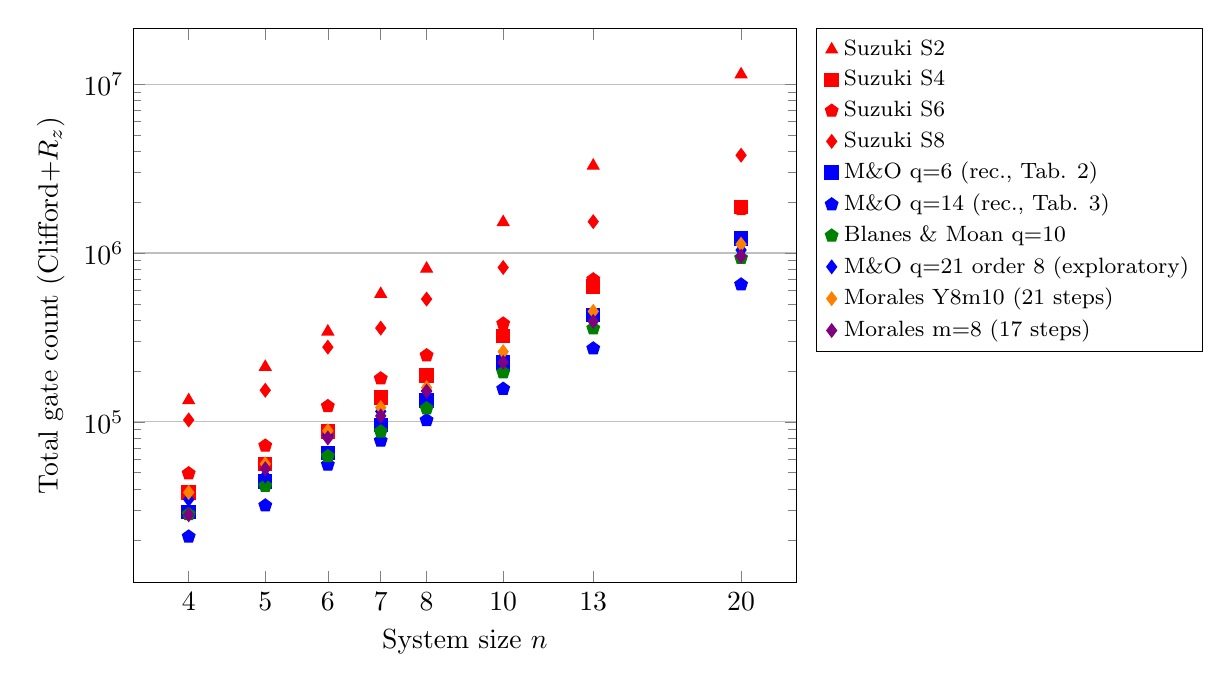
\begin{tikzpicture}
  \begin{loglogaxis}[
    width=10cm,
    xlabel={System size $n$},
    ylabel={Total gate count (Clifford+$R_z$)},
    xtick={4,5,6,7,8,10,13,20},
    xticklabels={4,5,6,7,8,10,13,20},
    ymajorgrids=true,
    legend pos=outer north east,
    legend cell align=left,
    legend style={font=\footnotesize},
  ]
    % r from power-law fit (extrapolation); one legend entry per series
    \addplot[only marks, red, mark=triangle*, mark size=2.4pt, mark options={solid, fill=red}] coordinates {
      (4,134208)
      (5,211440)
      (6,342432)
      (7,571536)
      (8,807168)
      (10,1523520)
    };
    \addlegendentry{Suzuki S2}
    % r from power-law fit (extrapolation); one legend entry per series
    \addplot[only marks, red, mark=triangle*, mark size=2.4pt, mark options={solid, fill=red}, forget plot] coordinates {
      (13,3289728)
      (20,11429760)
    };
    \addplot[only marks, red, mark=square*, mark size=2.4pt, mark options={solid, fill=red}] coordinates {
      (4,38160)
      (5,56180)
      (6,87768)
      (7,139496)
      (8,188256)
      (10,322240)
    };
    \addlegendentry{Suzuki S4}
    % r from power-law fit (extrapolation); one legend entry per series
    \addplot[only marks, red, mark=square*, mark size=2.4pt, mark options={solid, fill=red}, forget plot] coordinates {
      (13,633880)
      (20,1874080)
    };
    \addplot[only marks, red, mark=pentagon*, mark size=2.4pt, mark options={solid, fill=red}] coordinates {
      (4,49536)
      (5,72240)
      (6,123840)
      (7,180600)
      (8,247680)
      (10,381840)
    };
    \addlegendentry{Suzuki S6}
    % r from power-law fit (extrapolation); one legend entry per series
    \addplot[only marks, red, mark=pentagon*, mark size=2.4pt, mark options={solid, fill=red}, forget plot] coordinates {
      (13,697632)
      (20,1816320)
    };
    \addplot[only marks, red, mark=diamond*, mark size=2.4pt, mark options={solid, fill=red}] coordinates {
      (4,102640)
      (5,153960)
      (6,277128)
      (7,359240)
      (8,533728)
      (10,821120)
    };
    \addlegendentry{Suzuki S8}
    % r from power-law fit (extrapolation); one legend entry per series
    \addplot[only marks, red, mark=diamond*, mark size=2.4pt, mark options={solid, fill=red}, forget plot] coordinates {
      (13,1534468)
      (20,3797680)
    };
    \addplot[only marks, blue, mark=square*, mark size=2.4pt, mark options={solid, fill=blue}] coordinates {
      (4,29348)
      (5,44275)
      (6,65274)
      (7,95634)
      (8,133584)
      (10,225170)
    };
    \addlegendentry{M\&O q=6 (rec., Tab. 2)}
    % r from power-law fit (extrapolation); one legend entry per series
    \addplot[only marks, blue, mark=square*, mark size=2.4pt, mark options={solid, fill=blue}, forget plot] coordinates {
      (13,430859)
      (20,1219460)
    };
    \addplot[only marks, blue, mark=pentagon*, mark size=2.4pt, mark options={solid, fill=blue}] coordinates {
      (4,20916)
      (5,31955)
      (6,55776)
      (7,77273)
      (8,102256)
      (10,156870)
    };
    \addlegendentry{M\&O q=14 (rec., Tab. 3)}
    % r from power-law fit (extrapolation); one legend entry per series
    \addplot[only marks, blue, mark=pentagon*, mark size=2.4pt, mark options={solid, fill=blue}, forget plot] coordinates {
      (13,271908)
      (20,650720)
    };
    \addplot[only marks, green!50!black, mark=pentagon*, mark size=2.4pt, mark options={solid, fill=green!50!black}] coordinates {
      (4,28356)
      (5,41700)
      (6,62550)
      (7,87570)
      (8,120096)
      (10,195990)
    };
    \addlegendentry{Blanes \& Moan q=10}
    % r from power-law fit (extrapolation); one legend entry per series
    \addplot[only marks, green!50!black, mark=pentagon*, mark size=2.4pt, mark options={solid, fill=green!50!black}, forget plot] coordinates {
      (13,357786)
      (20,934080)
    };
    \addplot[only marks, blue, mark=diamond*, mark size=2.4pt, mark options={solid, fill=blue}] coordinates {
      (4,34720)
      (5,47740)
      (6,83328)
      (7,115444)
      (8,152768)
      (10,243040)
    };
    \addlegendentry{M\&O q=21 order 8 (exploratory)}
    % r from power-law fit (extrapolation); one legend entry per series
    \addplot[only marks, blue, mark=diamond*, mark size=2.4pt, mark options={solid, fill=blue}, forget plot] coordinates {
      (13,428792)
      (20,1041600)
    };
    \addplot[only marks, orange, mark=diamond*, mark size=2.4pt, mark options={solid, fill=orange}] coordinates {
      (4,38192)
      (5,56420)
      (6,88536)
      (7,121520)
      (8,159712)
      (10,260400)
    };
    \addlegendentry{Morales Y8m10 (21 steps)}
    % r from power-law fit (extrapolation); one legend entry per series
    \addplot[only marks, orange, mark=diamond*, mark size=2.4pt, mark options={solid, fill=orange}, forget plot] coordinates {
      (13,451360)
      (20,1128400)
    };
    \addplot[only marks, violet, mark=diamond*, mark size=2.4pt, mark options={solid, fill=violet}] coordinates {
      (4,28160)
      (5,52800)
      (6,80256)
      (7,108416)
      (8,152064)
      (10,225280)
    };
    \addlegendentry{Morales m=8 (17 steps)}
    % r from power-law fit (extrapolation); one legend entry per series
    \addplot[only marks, violet, mark=diamond*, mark size=2.4pt, mark options={solid, fill=violet}, forget plot] coordinates {
      (13,393536)
      (20,957440)
    };
  \end{loglogaxis}
\end{tikzpicture}
